%
% modeling.tex (LateX)
% 
% Objetivo: Capítulo sobre a etapa de modelagem do relatório de qualificação de doutorado.
% 
% Versão 1.0
% 
% Site: http://www.dirackslounge.online
% 
% Programador: Rodolfo A. C. Neves (Dirack) 16/10/2019
% 
% Email: rodolfo_profissional@hotmail.com
% 
% Licença: GPL-3.0 <https://www.gnu.org/licenses/gpl-3.0.txt>.

\chapter{MODELAGEM: REFLETOR GAUSSIANO EM UM MEIO COM GRADIENTE LINEAR DE VELOCIDADE}
\label{cap5:modeling}

Geramos uma superfície de tempo de trânsito de reflexão para o modelo do refletor gaussiano (Figura \ref{fig:5.1})
através da modelagem Kirchhoff\footnote{Este experimento é um dos vários ``artigos reproduzíveis'' disponíveis no site
do pacote de processamento sísmico Madagascar em \url{http://www.ahay.org/wiki/Main_Page}. 
Foi originalmente concebido por Sergey Fomel e Roman Kazinnik (2013),
está disponível para ser reutilizado sobre a licensa de uso GPL-3.0 para software livre disponível
em \url{https://www.gnu.org/licenses/gpl-3.0.txt}.}\cite{fomel1}.
Neste modelo a velocidade cresce linearmente com a profundidade com o gradiente 0.5, partindo da velocidade inicial de
1.5Km/s. 

A modelagem é realizada diretamente no domínio do ponto médio comum x afastamento. São 161 receptores (161 afastamentos),
espaçados de 0.025Km; e 401 PMC's, espaçados em 0.025Km. A frequência pico da wavelet é 10Hz, com 1001 amostras no tempo, a
cada 0.004s.

A Figura \ref{fig:5.2} apresenta os dados modelados organizados em um ``cubo de dados'' (as amplitudes nas amostras registradas
são identificadas pela tripla PMC, afastamento e tempo). A Figura \ref{fig:5.3} apresenta o tempo de trânsito de reflexão para o
modelo do refletor gaussiano, em função do PMC e do afastamento, em um mapa chamado de ``superfície de tempo de trânsito''.

Os menores tempos de reflexão são os registrados próximo ao 
ápice da gaussiana em 5Km (tempos em azul na Figura \ref{fig:5.3}) pela maior proximidade com o refletor.
E por último apresentamos a seção de afastamento nulo (Figura \ref{fig:5.4}) para o mesmo modelo.

\begin{figure}[H]
\caption{Modelo de velocidades utilizado na modelagem Kirchhoff: Modelo do refletor gaussiano em um meio com
gradiente linear de velocidade (a velocidade cresce linearmente com a profundidade). A velocidade próximo 
a superfície do modelo é 1.5Km/s e o gradiente de velocidade é 0.5.}
\begin{center}
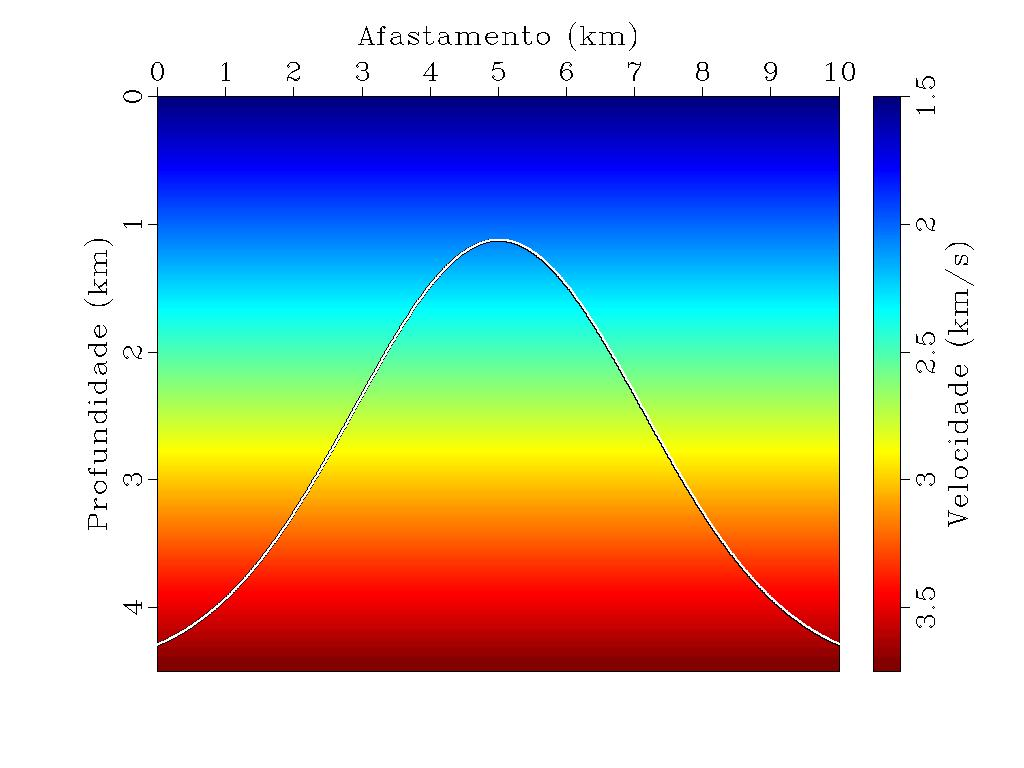
\includegraphics[scale=0.3]{images/dome.jpeg}
\vspace{-0.3cm}
\end{center}
\begin{center}
 Fonte: Do Autor.
\end{center}
\label{fig:5.1}
\end{figure}

\begin{figure}[htb]
\caption{Cubo de dados sísmicos modelados a partir da aplicação da modelagem Kirchoff ao modelo
do refletor gaussiano. O cubo apresenta os valores das amplitudes registradas em função das coordenadas do
ponto médio comum (PMC), afastamento e tempo.}
\begin{center}
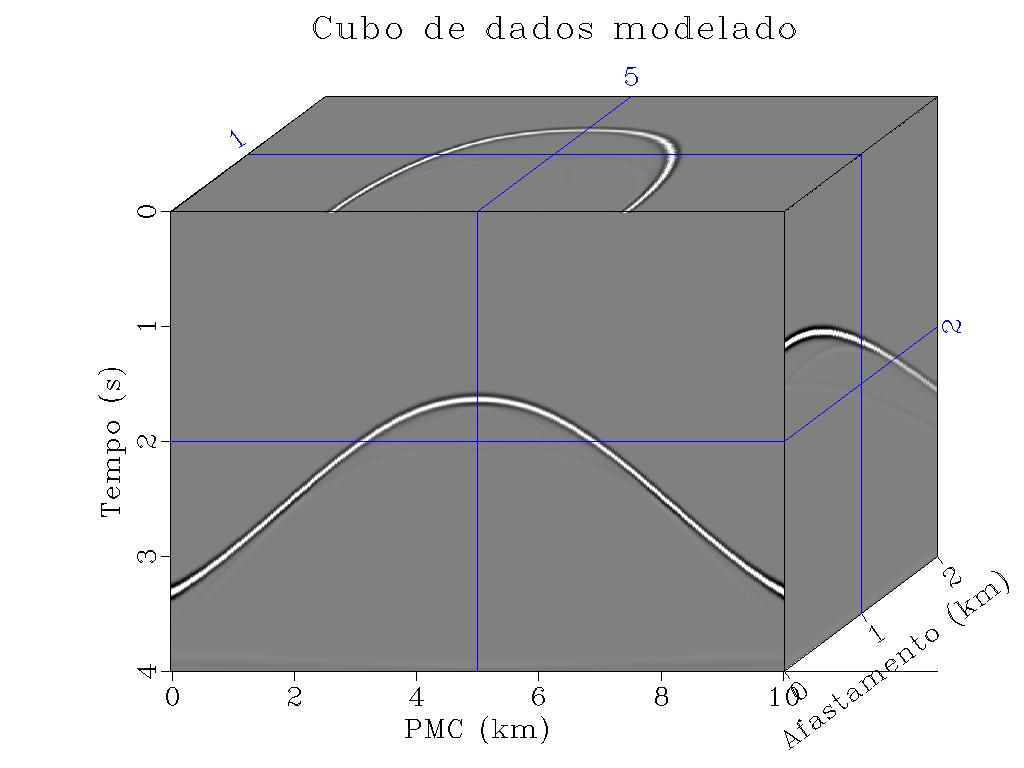
\includegraphics[scale=0.3]{images/dataCube.jpeg}
\vspace{-0.3cm}
\end{center}
\begin{center}
 Fonte: Do Autor.
\end{center}
\label{fig:5.2}
\end{figure}


%% Imagens dos offset gathers
\begin{figure}[htb]
\caption{Seção de afastamento constante extraída do cubo de dados. Esta seção representa um corte no
afastamento 0.5Km.}
\begin{center}
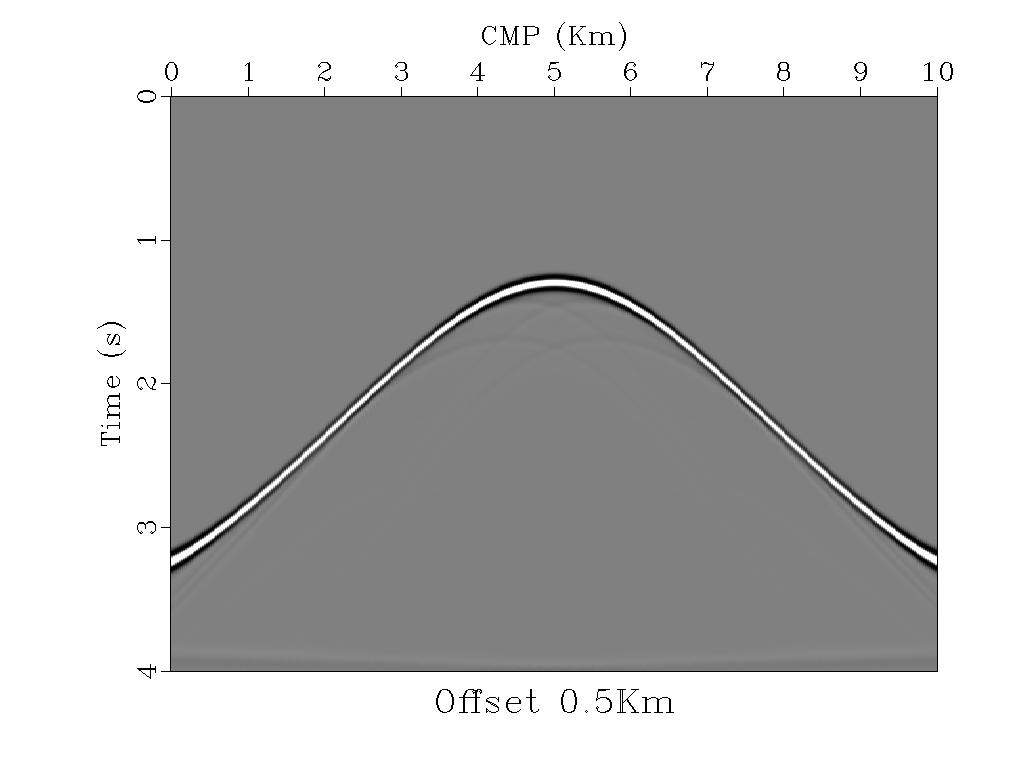
\includegraphics[scale=0.3]{images/off-40.jpeg}
\vspace{-0.3cm}
\end{center}
\begin{center}
 Fonte: Do Autor.
\end{center}
\label{fig:5.3}
\end{figure}

\begin{figure}[htb]
\caption{Seção de afastamento constante extraída do cubo de dados. Esta seção representa um corte no
afastamento 1.0Km.}
\begin{center}
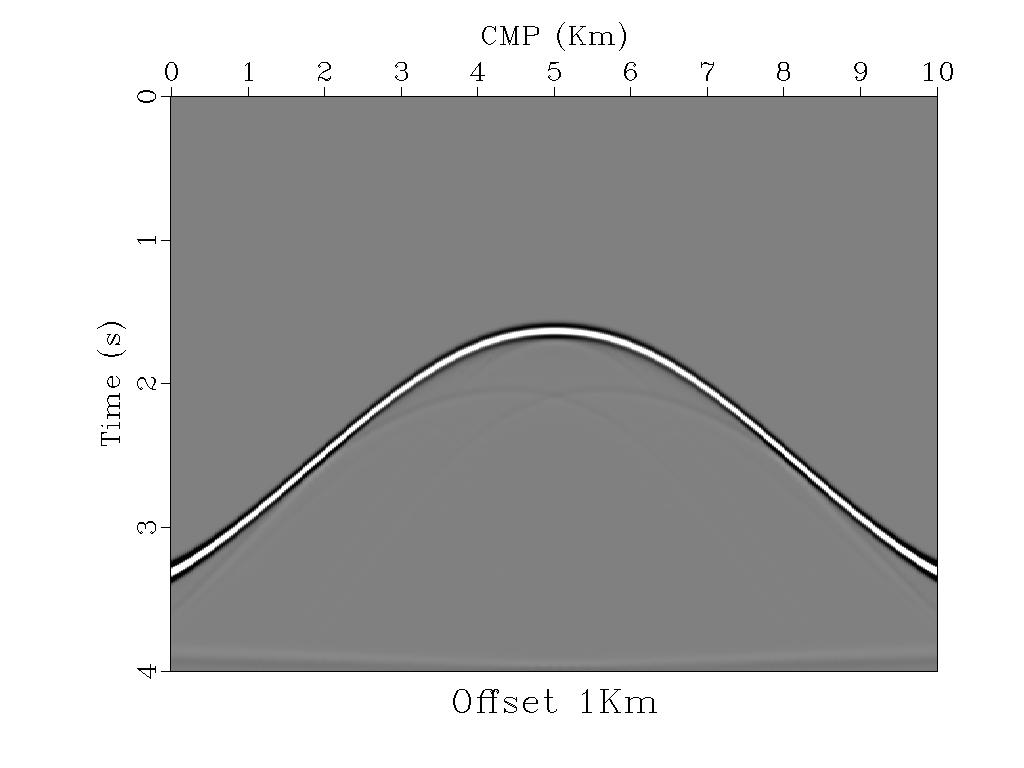
\includegraphics[scale=0.3]{images/off-80.jpeg}
\vspace{-0.3cm}
\end{center}
\begin{center}
 Fonte: Do Autor.
\end{center}
\label{fig:5.4}
\end{figure}

\begin{figure}[htb]
\caption{Seção de afastamento constante extraída do cubo de dados. Esta seção representa um corte no
afastamento 1.5Km.}
\begin{center}
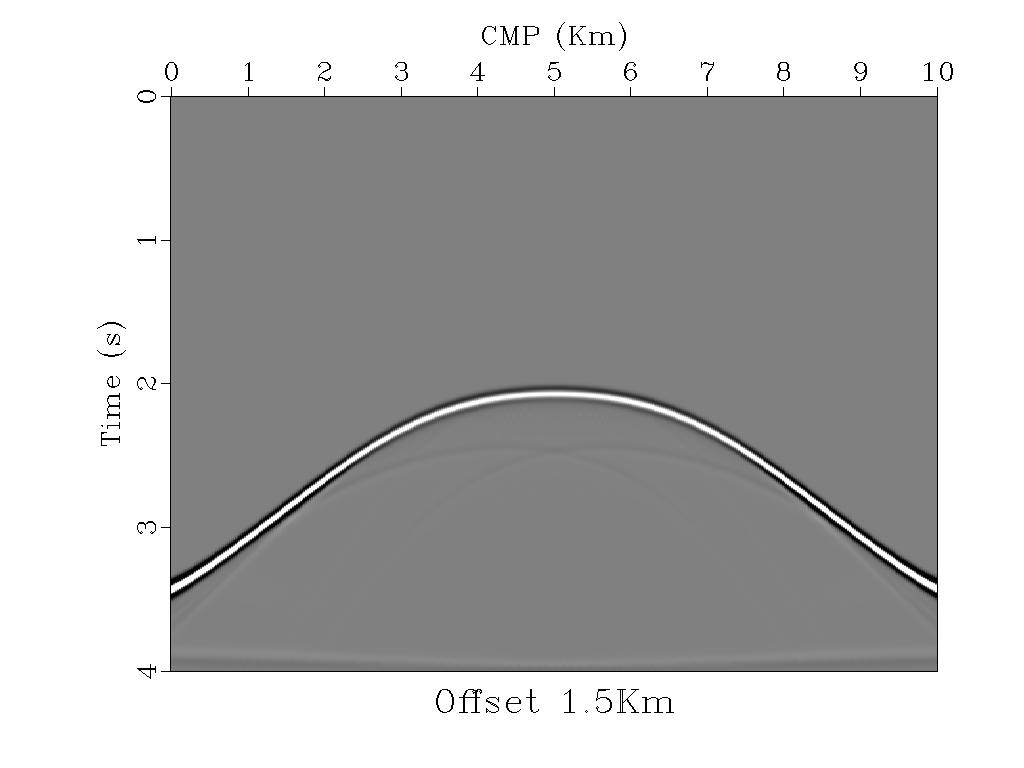
\includegraphics[scale=0.3]{images/off-120.jpeg}
\vspace{-0.3cm}
\end{center}
\begin{center}
 Fonte: Do Autor.
\end{center}
\label{fig:5.5}
\end{figure}



\begin{figure}[htb]
\caption{superfície de tempo de trânsito de reflexão para o modelo do refletor gaussiano.
O mapa apresenta os valores de tempo de trânsito registrados em função das coordenadas do
ponto médio comum (PMC) e afastamento.}
\begin{center}
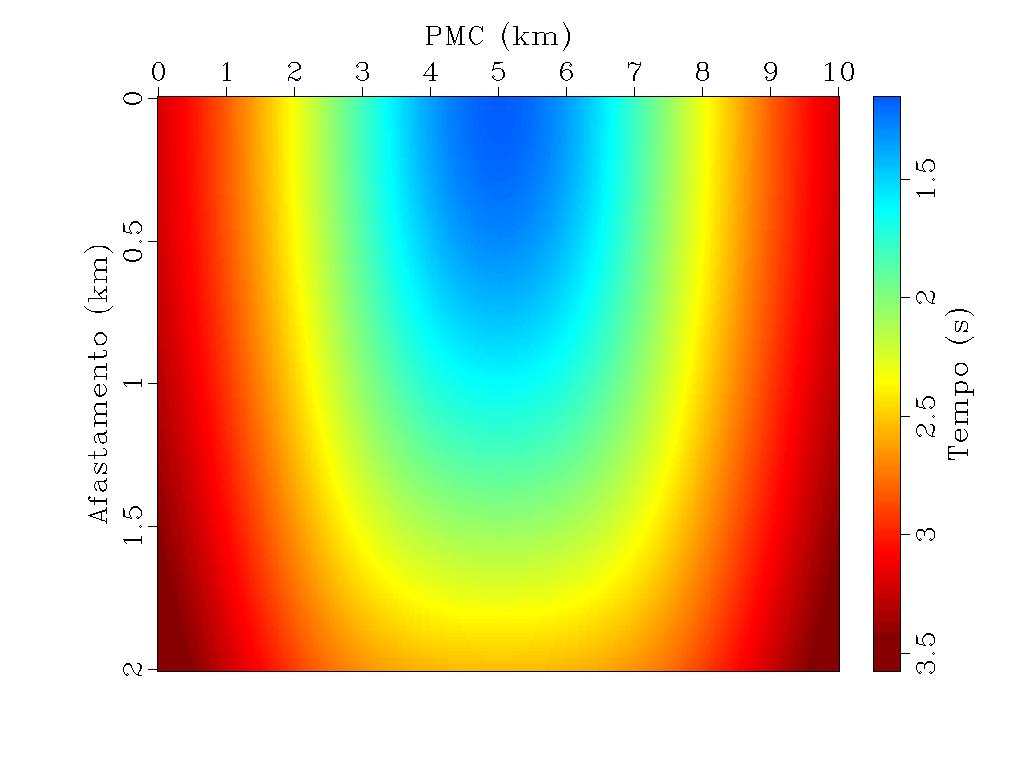
\includegraphics[scale=0.3]{images/reflectionSurface.jpeg}
\vspace{-0.3cm}
\end{center}
\begin{center}
 Fonte: Do Autor.
\end{center}
\label{fig:5.6}
\end{figure}

\begin{figure}[htb]
\caption{Seção de afastamento nulo para o modelo do refletor gaussiano.
A seção apresenta as amplitudes registradas em função das coordenadas do
ponto médio comum (PMC) e do tempo.}
\begin{center}
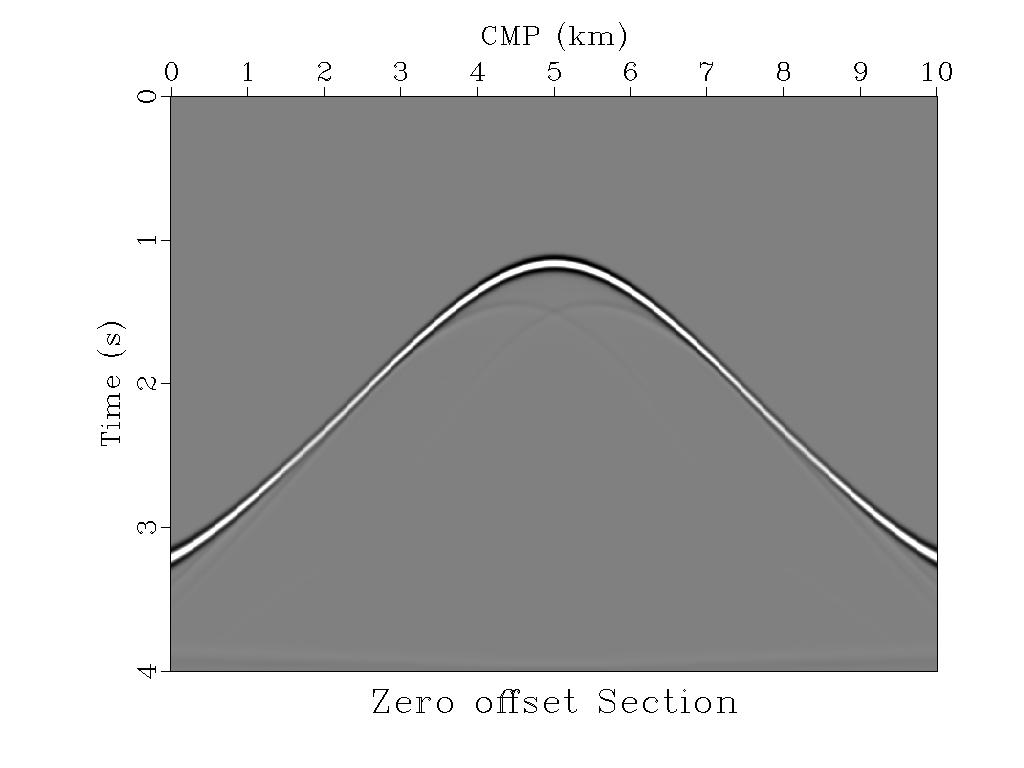
\includegraphics[scale=0.3]{images/zeroOffset.jpeg}
\vspace{-0.3cm}
\end{center}
\begin{center}
 Fonte: Do Autor.
\end{center}
\label{fig:5.7}
\end{figure}
